\part{Calculus}
\chapter{Single Variable Calculus}

applications of calculus involving parametric, polar and vector functions
polynomial approximations and convergence of series
asymptotic and unbounded behavior

\section{Limits}
\subsection{Informal Definition}
\begin{defn}{Intuitive definition of limit}{}
Suppose $f(x)$ is defined on some open interval that contains $a$, except possibly at $a$ itself. Then we write
\[ \lim_{x\to a} f(x) = L \]
and say ``the limit of $f(x)$, as $x$ approaches $a$, equals $L$" if we can make the values of $f(x)$ arbitrarily close to $L$ by restricting $x$ to be sufficiently close to $a$ (on either side of $a$) but not equal to $a$.
\end{defn}

\begin{defn}{Intuitive definition of one-sided limits}{}
We write $\lim_{x\to a^-}f(x)=L$ and say that the \textbf{left-hand limit} of $f(x)$ as $x$ approaches $a$ from the left is $L$.

Similarly, we write $\lim_{x\to a^+}f(x)=L$ and say that the \textbf{right-hand limit} of $f(x)$ as $x$ approaches $a$ from the right is $L$.
\end{defn}

For the limit $\lim_{x\to a}f(x)$ to exist,
\[ \lim_{x\to a^+}f(x) = \lim_{x\to a^-}f(x) \]

To indicate the behavior of vertical asymptotes or infinite limits, we use the notation $\lim_{x\to a}f(x)=\infty$.

\begin{defn}{Intuitive definition of infinite limit}{}
Let $f$ be a function defined on
both sides of $a$, except possibly at $a$ itself. Then
\[ \lim_{x\to a}f(x)=\infty \]
means that $f(x)$ can be made arbitrarily large by taking $x$ sufficiently close to, but not equal to $a$.
\end{defn}

\begin{remark}
This does not mean that we are regarding $\infty$ as a number, nor does it mean that the limit
exists; it simply expresses the particular way in which the limit does not exist: $f(x)$ can be made as large as we like by taking $x$ close enough to 0.
\end{remark}

A similar sort of limit, for functions that become large negative as $x$ gets close to $a$, is defined below.

\begin{defn}{}{}
Let $f$ be a function defined on both sides of $a$, except possibly at $a$ itself. Then
\[ \lim_{x\to a}f(x)=-\infty \]
means that $f(x)$ can be made arbitrarily large negative by taking $x$ sufficiently close to, but not equal to $a$.
\end{defn}

\begin{defn}{Vertical asymptote}{}
The vertical line $x=a$ is a \vocab{vertical asymptote} of $y=f(x)$ if at least one of the following statements is true:
\[ \lim_{x\to a}f(x)=\infty \quad \lim_{x\to a^-}f(x)=\infty \quad \lim_{x\to a^+}f(x)=\infty \]
\[ \lim_{x\to a}f(x)=-\infty \quad \lim_{x\to a^-}f(x)=-\infty \quad \lim_{x\to a^+}f(x)=-\infty \]
\end{defn}

\subsection{Limit Laws}
Let $f(x)$ and $g(x)$ be defined for all $x\neq a$ over some open interval containing $a$. Assume that $L$ and $M$ are real numbers such that $\lim_{x\to a}f(x)=L$ and $\lim_{x\to a}g(x)=M$, $c$ is a constant. Then each of the following statements holds.

\begin{itemize}
\item \textbf{Sum law}: The limit of a sum is the sum of the limits.
\[ \lim_{x\to a}(f(x)+g(x)) = \lim_{x\to a}f(x) + \lim_{x\to a}g(x) = L+M \]

\item \textbf{Difference law}: The limit of a difference is the difference of the limits.
\[ \lim_{x\to a}(f(x)-g(x)) = \lim_{x\to a}f(x) - \lim_{x\to a}g(x) = L-M \]

\item \textbf{Constant multiple law}: The limit of a constant times a function is the constant times the limit of the function.
\[ \lim_{x\to a}cf(x) = c\lim_{x\to a}f(x) = cL \]

\item \textbf{Product law}: The limit of a product is the product of the limits.
\[ \lim_{x\to a}(f(x)\cdot g(x)) = \lim_{x\to a}f(x) \cdot \lim_{x\to a}g(x) = L\cdot M \]

\item \textbf{Quotient law}: The limit of a quotient is the quotient of the limits.
\[ \lim_{x\to a}\frac{f(x)}{g(x)} = \frac{\lim_{x\to a}f(x)}{\lim_{x\to a}g(x)} = \frac{L}{M} \]
for $M \neq 0$.

\item \textbf{Power law}
\[ \lim_{x\to a}(f(x))^n = (\lim_{x\to a}f(x))^n = L^n \]
for every positive integer $n$.

\item \textbf{Root law}
\[ \lim_{x\to a}\sqrt[n]{f(x)} = \sqrt[n]{\lim_{x\to a}f(x)} = \sqrt[n]{L} \]
for all $L$ if $n$ is odd, and for $L\ge 0$ if $n$ is even.
\end{itemize}
\pagebreak

\subsection{Evaluating Limits}
Indeterminate forms of a limit include:
\[ \frac{0}{0} \quad \frac{\infty}{\infty} \quad 0 \times \infty \quad \infty - \infty \quad 0^0 \quad 1^{\infty} \quad \infty^0 \]
As long as limits are in indeterminate forms, they can still be evaluated.

Methods:
\begin{itemize}
\item Direct substitution

If $f$ is a polynomial or a rational function and $a$ is in the domain of $f$, then
\[ \lim_{x\to a}f(x)=f(a) \]

\item Cancel common factors
\item Multiply by the conjugate of the numerator or denominator
\end{itemize}

\begin{exmp}{}{}
Evaluate the following limit:
\[ \lim_{x\to 0} x^2\sin\brac{\frac{1}{x}} \]
\end{exmp}

\begin{proof}[Solution]
If we plot the graph of the function out, we see that we can try to find two functions to apply Squeeze Theorem.

Notice that \[ -1 \le \sin\brac{\frac{1}{x}} \le 1 \]
and hence
\[ -x^2 \le x^2\sin\brac{\frac{1}{x}} \le x^2 \]
thus $x^2$ and $-x^2$ are the two functions that ``sandwich" the given function.

Since $\lim_{x\to 0}x^2=0$ and $\lim_{x\to 0}-x^2=0$, applying Squeeze Theorem gives us 
\[ \lim_{x\to 0} x^2\sin\brac{\frac{1}{x}} = 0 \]
\end{proof}

\begin{exmp}{}{}
Evaluate the following limit:
\[ \lim_{x\to 3}\frac{-4x}{x-3} \]
\end{exmp}

\begin{proof}[Solution]
Approaching from the left side,
\[ \lim_{x\to 3^-}\frac{-4x}{x-3} = +\infty \]
Approaching from the right side,
\[ \lim_{x\to 3^+}\frac{-4x}{x-3} = -\infty \]
Since $\lim_{x\to 3^-}\dfrac{-4x}{x-3} \neq \lim_{x\to 3^+}\dfrac{-4x}{x-3}$, the limit does not exist.
\end{proof}

\begin{thrm}{}{}
If $f(x) \le g(x)$ when $x$ is near $a$ (except possibly at $a$) and the limits of $f$ and $g$ both exist as $x$ approaches $a$, then
\[ \lim_{x\to a}f(x) \le \lim_{x\to a}g(x) \]
\end{thrm}

\begin{thrm}{Squeeze theorem}{}
Suppose that $g(x) \ge f(x) \ge h(x)$ for all $x$ in some open interval containing $c$ except possibly at $c$ itself. If $\lim_{x\to c} g(x) = L = \lim_{x\to c} h(x)$, then $\lim_{x\to c} f(x) = L$.
\end{thrm}

\begin{proof}
This can be proven using the epsilon-delta definition of limits.

Let $\epsilon > 0$ be given. We are done if we find a $\delta > 0$ such that $|f(x)-L| < \epsilon$ whenever $0 < |x-c| < \delta$.

Since $\lim_{x\to c} g(x) = L$, by definition of limits, there exists some $\delta_1 > 0$ such that for all $0 < |x-c| < \delta_1$, $|g(x)-L| < \epsilon$.
Thus, 
\[ -\epsilon < g(x)-L < \epsilon \quad \text{for all } 0 < |x-c| < \delta_1 \]
so
\begin{equation*}\tag{1}
L-\epsilon < g(x) < L + \epsilon \quad \text{for all } 0 < |x-c| < \delta_1
\end{equation*}
Similarly, since $\lim_{x\to c} h(x) = L$, by definition of limits, there exists some $\delta_2 > 0$ such that
\begin{equation*}\tag{2}
L-\epsilon < h(x) < L + \epsilon \quad \text{for all } 0 < |x-c| < \delta_2
\end{equation*}
Additionally, since $g(x) \le f(x) \le h(x)$ for all $x$ in some open interval containing $c$, there exists some $\delta_3 > 0$ such that for 
\begin{equation*}\tag{3}
g(x) \le f(x) \le h(x) \quad \text{for all } 0 < |x-c| < \delta_3
\end{equation*}
Now, we choose $\delta = \min(\delta_1, \delta_2, \delta_3)$. Then by (1), (3), and (2), we have 
\[ L-\epsilon < g(x) \le f(x) \le h(x) < L + \epsilon \quad \text{for all } 0 < |x-c| < \delta. \]
Therefore, $-\epsilon < f(x)-L < \epsilon$ for all $0 < |x-c| < \delta$, so
\[ |f(x)-L| < \epsilon \quad \text{for all } 0 < |x-c| < \delta. \]
Hence, by definition of limits, $\lim_{x\to c} f(x) = L$.
\end{proof}

\begin{thrm}{L'H\^{o}pital's Rule}{}
Let $f(x)$ and $g(x)$ be differentiable on an interval $I$ containing $a$, and that $g^\prime(a) \neq 0$ on $I$ for $x \neq a$. Suppose that
\[ \lim_{x\to a}\frac{f(x)}{g(x)} \]
is in an indeterminate form. 

Then as long as the limits exist, we have 
\[ \lim_{x\to a}\frac{f(x)}{g(x)} = \lim_{x\to a}\frac{f^\prime(x)}{g^\prime(x)}. \]
\end{thrm}

\begin{proof}

\end{proof}
\pagebreak

% uniqueness of the limit

\subsection{Precise Definition of a Limit}
The intuitive definition of a limit given above is inadequate because such phrases as ``$x$ is close to 2" and ``$f(x)$ gets closer and closer to $L$" are vague. In order to be able to prove limits conclusively, we must make the definition of a limit precise.

\begin{defn}{Epsilon--delta definition of limit}{}
Let $f(x)$ be a function defined on an open interval around $x_0$. We say that the limit of $f(x)$ as $x$ approaches $x_0$ is $L$, i.e. 
\[ \lim_{x \to x_0} f(x) = L \]
if $\forall \epsilon > 0$, there exists $\delta > 0$ such that $\forall x \in \RR$, 
\[ \absolute{x-x_0}<\delta \implies \absolute{f(x)-L}<\epsilon \] 
\end{defn} 

Visualising this graphically, 
\begin{figure}[H]
	\centering
	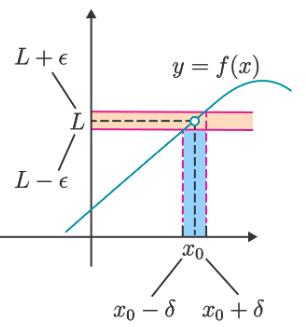
\includegraphics[width=6cm]{images/Epsilon_delta_definition.png}
\end{figure}
As $\epsilon$ becomes smaller and smaller, there always exists a $\delta$ that satisfies the property that for any $x$ in the open interval $(x_0-\delta,x_0+\delta)$, the value of $f(x)$ lies in the interval $(L-\epsilon, L+\epsilon)$.

\begin{exmp}{}{} 
Prove that \[ \lim_{x \to 3} 2x+4 = 10. \] \end{exmp}

Before the proof, we work backwards to find the value of $\delta$ in terms of $\epsilon$ and $x_0$, which we then declare in our proof.

$\forall \epsilon > 0$, $\exists \delta > 0$, $\forall x \in \RR$,
\[ |x-3| < \delta \implies |f(x)-10| < \epsilon \]
Let $\epsilon > 0$ be given.
\[ |f(x)-10| = |2x+4-10| = |2x-6| = 2|x-3| < \epsilon \]
Notice $|x-3| < \dfrac{\epsilon}{2}$. We can thus define $\delta \coloneqq \dfrac{\epsilon}{2}$. We now write our proof.

\begin{proof}
Let $\epsilon > 0$ be given. Choose $\delta = \dfrac{\epsilon}{2}$.

Then $\forall x \in \RR$, 
\begin{align*}
|x-3| &< \delta = \frac{\epsilon}{2} \\
2|x-3| &< \epsilon \\
|2x-6| &< \epsilon \\
|2x+4-10| &< \epsilon \\
|f(x)-10| &< \epsilon
\end{align*}
\end{proof}

\begin{exmp}{}{}
Use the formal definition of the limit to verify that 
\[ \lim_{x \to 3} \sqrt{2x+3} = 3. \]
\end{exmp}

We must prove that $\forall \epsilon > 0$, $\exists \delta > 0$ such that $\sqrt{2x+3} - 3 < \epsilon$ whenever $|x-3|<\delta$.
\begin{align*}
\sqrt{2x+3} - 3 &= \absolute{\frac{(2x+3)-3^2}{\sqrt{2x+3} + 3}} = \absolute{\frac{2x-6}{\sqrt{2x+3} + 3}} \\
&\le \absolute{\frac{2(x-3)}{3}} \\
&= \frac{2}{3} \absolute{x-3} < \frac{2}{3} \delta
\end{align*}
Hence, we can define 
\[ \epsilon \coloneqq \frac{2}{3} \delta \]
which we can use in our proof.
\pagebreak

\subsection{Important Limits}
\begin{equation}
\lim_{x \to 0} \frac{\sin x}{x} = 1
\end{equation}
\begin{proof}
This can be proven using the squeeze theorem, which will be discussed later.
\end{proof}

\begin{equation}
\lim_{x \to 0} \frac{1-\cos x}{x} = 0
\end{equation}
\begin{proof}
This can be proven using the squeeze theorem, which will be discussed later.
\end{proof}

\begin{equation}
\lim_{x\to 0} \frac{\arcsin x}{x} = 1
\end{equation}

\begin{equation}
\lim_{x\to \pm\infty} \brac{1+\frac{1}{x}}^x=e
\end{equation}
\pagebreak

\subsection{Continuity}
\begin{defn}{Continuity}{}
A function $f(x)$ is continuous at $x=a$ if 
\[ \lim_{x\to a} f(x)=f(a) \]
A function is said to be continuous on the interval  $[a,b]$ if it is continuous at each point in the interval.
\end{defn}
Note that this definition is also implicitly assuming that both $f(a)$ and $\lim_{x\to a}f(x)$ exist. If either of these do not exist the function will not be continuous at $x=a$.

This definition can be turned around into the following fact.
\begin{corollary}
If $f(x)$ is continuous at $x=a$ then
\[ \lim_{x \to a} f(x) = f(a) \quad \lim_{x \to a^-} f(x) = f(a) \quad \lim_{x \to a^+} f(x) = f(a) \]
\end{corollary}

A nice consequence of continuity is the following fact.
\begin{corollary}
If $f(x)$ is continuous at $x=b$ and $\lim_{x\to a}g(x)=b$ then
\[ \lim_{x \to a} f(g(x)) = f(\lim_{x \to a} g(x)) \]
\end{corollary}

\begin{exmp}{}{}
Evaluate the following limit:
\[ \lim_{x \to 0} e^{\sin x} \]
\end{exmp}

\begin{proof}[Solution]
Since we know that exponentials are continuous everywhere we can use the fact above.
\[ \lim_{x \to 0} e^{\sin x} = e^{\lim_{x \to 0} \sin x} = e^0 = \boxed{1} \]
\end{proof}

Another very nice consequence of continuity is the Intermediate Value Theorem.
\begin{thrm}{Intermediate Value Theorem}{}
Suppose that $f(x)$ is continuous on $[a,b]$ and let $M$ be any number between $f(a)$ and $f(b)$. Then there exists $c \in (a,b)$ such that $f(c)=M$.
\end{thrm}
All the Intermediate Value Theorem is really saying is that a continuous function will take on all values between $f(a)$ and $f(b)$.
\pagebreak

\section{Derivative}
\subsection{Definitions}
\begin{defn}{Derivative}{} 
The \vocab{derivative} of $f(x)$ with respect to $x$, denoted by $f^\prime(x)$, is defined as 
\begin{equation} f^\prime (x) = \lim_{h \to 0} \frac{f(x+h)-f(x)}{h}.
\end{equation}
\end{defn}

\begin{defn}{Differentiability}{} 
$f(x)$ is \vocab{differentiable} at $x_0$ if $f^\prime(x_0)$ exists. 

$f(x)$ is \vocab{differentiable} on an interval if the derivative exists for each and every point in the interval.
\end{defn}

\begin{defn}{Continuity}{} 
$f(x)$ is \vocab{continuous} at $x_0$ if $f(x)$ is differentiable at $x=x_0$.
\end{defn}

\begin{proof}
\begin{align*}
\lim_{x \to x_0} (f(x) - f(x_0)) &= \lim_{x \to x_0} \frac{(f(x) - f(x_0))(x-x_0)}{x - x_0}\\
&= \lim_{x \to x_0} \frac{f(x) - f(x_0)}{x - x_0} \cdot (x-x_0)\\
&= f^\prime (x_0) \cdot 0 = 0
\end{align*}
\end{proof}

\subsection{Theorems}
% move this to real analysis
\begin{thrm}{Extreme Value Theorem}{}
For a function $f$ continuous on $[a,b]$, it attains its maximum and minimum values on $[a,b]$.
\end{thrm}

\begin{proof}
We prove the case that $f$ attains its maximum value on $[a,b]$.

Since $f$ is continuous on $[a,b]$, we know it must be bounded on $[a,b]$ by the Boundedness Theorem. Let $M = \sup f$.

If there is some $c \in [a,b]$ where $f(c)=M$ there is nothing more to show -- $f$ attains its maximum on $[a,b]$.

Suppose otherwise, that there is no such $c$. Then $f(x)<M$ for all $x \in [a,b]$.

We define a new function $g$ by 
\[ g(x) = \frac{1}{M-f(x)}. \]

Note that $g(x)>0$ for every $x \in [a,b]$ and $g$ is continuous on $[a,b]$, and thus also bounded on this interval, again by the Boundedness theorem.

Given that $g$ is bounded on $[a,b]$, there must exist some $K>0$ such that $g(x) \le K$ for every $x \in [a,b]$.

Consequently,
\[ \frac{1}{M-f(x)} \le K \implies f(x) \le M - \frac{1}{K} \]
for every $x \in [a,b]$. This contradicts the assumption that $M$ is the least upper bound.

That leaves as the only possibility that there is some $c$ in $[a,b]$ where $f(c)=M$. That is to say, $f$ attains its maximum on $[a,b]$.

The proof that $f$ attains its minimum on the same interval is argued similarly and is left as an exercise for the reader.
\end{proof}

\begin{thrm}{Mean Value Theorem}{}
Let $f:[a,b]\to\RR$ be a continuous function on the closed interval $[a,b]$ and differentiable on the open interval $(a,b)$. Then there exists $c \in (a,b)$ such that 
\[ f^\prime(c)=\frac{f(b)-f(a)}{b-a}. \]
\end{thrm}

\begin{figure}[H]
    \centering
    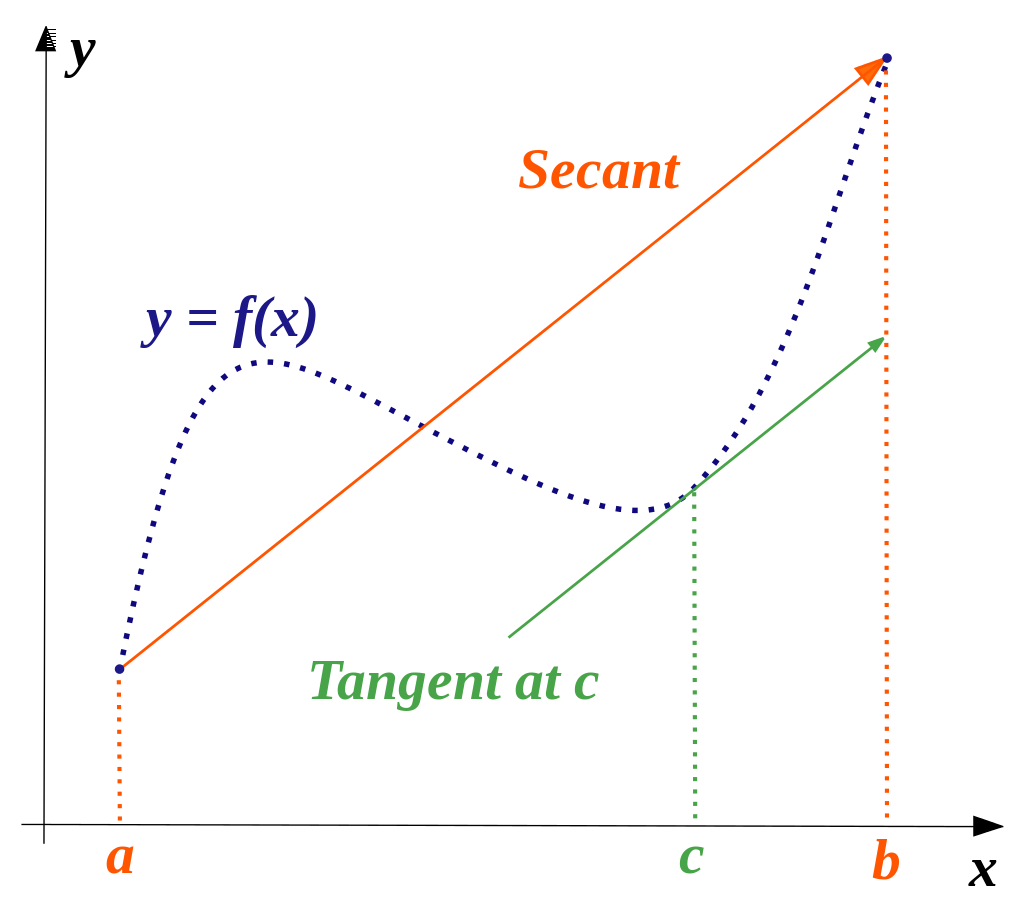
\includegraphics[width=8cm]{images/mean_value_thrm.png}
    \caption{Mean value theorem}
\end{figure}

\begin{thrm}{Rolle's Theorem}{}
Let $f:[a,b]\to\RR$ be a continuous function on the closed interval $[a,b]$ and differentiable on the open interval $(a,b)$, and $f(a)=f(b)$. Then there exists $c \in (a,b)$ such that 
\[ f^\prime(c)=0. \]
\end{thrm}
\begin{remark}
Rolle's Theorem is simply a special case of the Mean Value Theorem, where $f(a)=f(b)$.
\end{remark}

\subsection{Differentiation rules}
For a constant $c$ and functions $f$ and $g$, the following rules hold.

\begin{itemize}
\item \textbf{Scalar multiplication}
\[ (cf)^\prime = cf^\prime \]

\item \textbf{Addition rule}
\[ (f+g)^\prime = f^\prime + g^\prime \]

\begin{proof}
\begin{align*}
(f + g)^\prime (x) &= \lim_{h \to 0} \frac{(f+g)(x+h) - (f+g)(x)}{h}\\
&= \lim_{h \to 0} \frac{f(x+h) + g(x+h) - f(x) - g(x)}{h}\\
&= \lim_{h \to 0} \left[ \frac{f(x+h) - f(x)}{h} + \frac{g(x+h) - g(x)}{h} \right] \\
&= \lim_{h \to 0} \frac{f(x+h) - f(x)}{h} + \lim_{h \to 0} \frac{g(x+h) - g(x)}{h}\\
&= f^\prime (x) + g^\prime (x)
\end{align*}
\end{proof}

\item \textbf{Power rule}
\[ \dv{x} x^n = n x^{n-1} \]

\begin{proof}
Using implicit differentiation,
\begin{align*}
y &= x^n \\
\ln y &= \ln x^n \\
\ln y &= n \ln x \\
\frac{y^\prime}{y} &= n \frac{1}{x}
\end{align*}
\[ y^\prime = y \frac{n}{x} = x^n \brac{\frac{n}{x}} = n x^{n-1} \]
\end{proof}

\item \textbf{Product rule}
\[ (fg)^\prime = f^\prime g + f g^\prime \]

\begin{proof}
\begin{align*}
(fg)^\prime (x) &= \lim_{h \to 0} \frac{(fg)(x+h) - (fg)(x)}{h}\\
&= \lim_{h \to 0} \frac{f(x+h) g(x+h) - f(x) g(x)}{h}\\
&= \lim_{h \to 0} \frac{f(x+h) g(x) - f(x) g(x) + f(x+h) g(x+h) - f(x+h) g(x)}{h}\\
&= \lim_{h \to 0} \frac{f(x+h) g(x) - f(x) g(x)}{h} + \lim_{h \to 0} \frac{f(x+h) g(x+h) - f(x+h) g(x)}{h}\\
&= \lim_{h \to 0} \frac{f(x+h) - f(x)}{h}g(x) + \lim_{h \to 0} \frac{g(x+h) - g(x)}{h}f(x+h)\\
&= \left[\lim_{h \to 0} \frac{f(x+h) - f(x)}{h}\right] g(x) + \left[\lim_{h \to 0} \frac{g(x+h) - g(x)}{h}\right] f(x)\\
&= f^\prime (x) g(x) + f(x) g^\prime (x)
\end{align*}
\end{proof}

\item \textbf{Quotient rule}
\[ \brac{\frac{f}{g}}^\prime = \frac{f^\prime g - fg^\prime}{g^2} \] 

\begin{proof}
\begin{align*}
\left[\frac{f(x)}{g(x)}\right]^\prime &= \lim_{h \to 0} \frac{\frac{f(x+h)}{g(x+h)} - \frac{f(x)}{g(x)}}{h}\\
&= \lim_{h \to 0} \frac{1}{h} \frac{f(x+h) g(x) - f(x) g(x+h)}{g(x+h) g(x)}\\
&= \lim_{h \to 0} \frac{1}{h} \frac{f(x+h) g(x) - f(x) g(x) + f(x) g(x) - f(x) g(x+h)}{g(x+h) g(x)}\\
&= \lim_{h \to 0} \frac{1}{g(x+h) g(x)} \left[ \frac{f(x+h)g(x) - f(x)g(x)}{h} + \frac{f(x)g(x) - f(x)g(x+h)}{h} \right] \\
&= \lim_{h \to 0} \frac{1}{g(x+h) g(x)} \left[ g(x)\frac{f(x+h) - f(x)}{h} - f(x)\frac{g(x) + g(x+h)}{h} \right] \\
&= \frac{1}{g^2(x)} [g(x) f^\prime(x) - f(x) g^\prime(x)] \\
&= \frac{f^\prime(x) g(x) - f(x) g^\prime(x)}{g^2(x)}
\end{align*}
\end{proof}

\item \textbf{Chain rule}
\begin{thrm}{Chain rule}{} 
If $f$ and $g$ are both differentiable functions and we define $F(x) = (f \circ g)(x)$, then the derivative of $F(x)$ is
\begin{equation}
F^\prime (x) = f^\prime(g(x)) g^\prime(x) 
\end{equation} 
\end{thrm}
\begin{proof}

\end{proof}
\end{itemize}

\subsection{Implicit differentiation}
\textbf{Implicit differentiation} simply means differentiating both sides of the equation with respect to a variable.

\subsection{Taylor Series}
A function $f$ can be represented as a Taylor series about position $a$ if
\begin{itemize}
\item it is continuous near $a$ and
\item all of its derivatives are continuous near $a$
\end{itemize}

Using the notation $\Delta x = x-a$:
\[ f(x)=f(a)+\Delta xf^\prime(a)+\frac{\Delta x}{2!}f^{\prime\prime}(a) + \frac{\Delta x}{3!}f^{(3)}(a) + \cdots + \frac{\Delta x}{n!}f^{(n)}(a) + \cdots \]

If infinitely many terms are used, this approximation is exact near $a$.

If all terms of order $n$ and above are discarded then the error is approximately proportional to $\Delta x^n$ (assuming that $\Delta x$ is small). Then the approximation is said to be $n$-th order accurate. For example, a third order accurate approximation for $f(x)$ has error proportional to $\Delta x^3$. We say that  the error is of order $\Delta x^3$ or $O(\Delta x^3)$.
\[ f(x)=f(a)+\Delta xf^\prime(a)+\frac{\Delta x}{2!}f^{\prime\prime}(a) + O(\Delta x^3) \]


Maclaurin series,  determine radius and interval
of convergence of a power series

\subsection{Newton's Method}
In this section we are going to look at a method for approximating solutions to equations.

\begin{figure}[H]
    \centering
    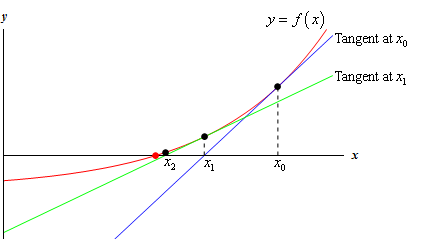
\includegraphics[width=10cm]{images/newton_method.png}
\end{figure}

Suppose that we want to approximate the solution to $f(x)=0$. Suppose that we have somehow found an initial rough approximation to the solution: $x=x_0$. The tangent line to $f(x)$ at $x=x_0$ is
\[ y = f(x_0) + f^\prime(x_0)(x-x_0) \]

This tangent line crosses the $x$-axis much closer to the actual solution to the equation than $x_0$ does. Let the tangent at $x_0$ intersect $x$-axis at $x_1$. We use this point as our new approximation to the solution. $x_1$ is given by:
\[ x_1 = x_0 - \frac{f(x_0)}{f^\prime(x_0)} \]

Repeat the process; form up the tangent line at $x_1$ and use its root $x_2$ as a new approximation:
\[ x_2 = x_1 - \frac{f(x_1)}{f^\prime(x_1)} \]

Here is the general Newton's Method:
\begin{thrm}{Newton's Method}{}
If $x_n$ is an approximation of a solution of $f(x)=0$ and if $f^\prime(x_n) \neq 0$, then the next approximation is given by
\[ x_{n+1} = x_n - \frac{f(x_n)}{f^\prime(x_n)} \]
\end{thrm}
\pagebreak

\section{Integral}
\subsection{Definition}
We use the \textbf{Riemann} definition of an integral:
\begin{defn}{Integral}{}
An integral is defined as an infinite sum over an interval.
\begin{equation}
\int_a^b f(x) \dd{x} = \lim_{n \to \infty} \sum_{i=1}^n f(x_i) \Delta x
\end{equation}
\end{defn}

A Riemann sum is an approximation of an integral by a finite sum.

Let $f$ be defined on the closed interval $[a,b]$ and let $\Delta x$ be a partition of $[a,b]$, with
\[ a=x_1 < x_2 < \cdots < x_n < x_{n+1}=b.\]

Let $\Delta x_i$ denote the length of the $i$th subinterval $[x_i,x_{i+1}]$ and let $c_i$ denote any value in the $i$th subinterval.

The sum
\[ \sum_{i=1}^n f(c_i)\Delta x_i\]
is a Riemann sum of $f$ on $[a,b]$.

As the subinterval becomes infinitesimally small, 
\begin{equation} \int _{a}^{b}f(x) \dd{x} = \lim _{\Delta x \to 0} \sum _{i=1}^{n} f(x_{i}) \Delta x_{i} \end{equation}

\begin{figure}[H]
	\centering
	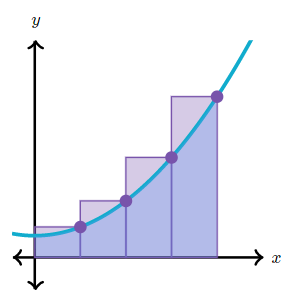
\includegraphics[width=8cm]{Riemanns_sums}
\end{figure}

Given a graph $y=f(x)$, and we want to find the integral on the $x$-interval $[0,1]$.

Split the interval $[0,1]$ into $n$ equal subintervals 
\[\sqbrac{0, \frac{1}{n}}, \sqbrac{\frac{1}{n}, \frac{2}{n}}, \cdots, \sqbrac{\frac{n-1}{n}, 1}.\]

Consider the height of the rectangles. We take the right value. Hence for the $k$th subinterval $\sqbrac{\dfrac{k-1}{n}, \dfrac{k}{n}}$ where $k=1,\dots,n$, height of rectangle is $f\brac{\dfrac{k}{n}}$.

Area of $k$th rectangle is \[ \frac{1}{n} \cdot f\brac{\frac{k}{n}}.\]
Therefore, the integral is obtained by summing up the area of $n$ rectangles, which gives us
\begin{equation} \int_{0}^{1} f(x) \dd{x} = \lim_{n \to \infty} \sum_{k=1}^{n} \frac{1}{n} f\brac{\frac{k}{n}} \end{equation}
where there are infinitely many rectangles, i.e. $n \to \infty$.

\begin{thrm}{Fundamental Theorem of Calculus}{}
The fundamental theorem of (single variable) calculus states that if $f^\prime$ is continuous on $[a,b]$, then the integral of the derivative across the bounds is equal to the original function at the bounds:
\begin{equation}
\int_a^b f^\prime(x) \dd{x} = f(b)-f(a)
\end{equation}
or equivalently,
\begin{equation}
\dv{x} \int_{a}^{x} f(s) \dd{s} = f(x)
\end{equation}
\end{thrm}

% https://www2.clarku.edu/faculty/djoyce/ma121/FTCproof.pdf

Using the definition of the derivative, we differentiate the following integral:
\begin{align*}
\dv{x} \int_{a}^{x} f(s) \dd{s} &= \lim_{h \to 0} \frac{\int_{a}^{x+h} f(s) \dd{s} - \int_{a}^{x} f(s) \dd{s}}{h}\\
&= \lim_{h \to 0} \frac{\int_{x}^{x+h} f(s) \dd{s}}{h}\\
&= \lim_{h \to 0} \frac{h f(x)}{h}\\
&= f(x)
\end{align*}
% https://math.libretexts.org/Bookshelves/Calculus/Calculus_3e_(Apex)/05%3A_Integration/5.04%3A_The_Fundamental_Theorem_of_Calculus

\subsection{Integration rules}
For constant $k\in\RR$ and functions $f(x)$ and $g(x)$, the following rules hold.
\begin{itemize}
\item \textbf{Sum and difference rule}
\[ \int f(x)\pm g(x) \dd{x} = \int f(x) \dd{x} \pm \int g(x) \dd{x} \]

\item \textbf{Scalar multiplication}
\[ \int kf(x) \dd{x} = k\int f(x) \dd{x} \]

\item \textbf{Power rule}
\[ \int x^n \dd{x} = \frac{x^{n+1}}{n+1} + C \]

\item \textbf{Constant rule}
\[ \int a\dd{x} = ax + C \]
\end{itemize}

\subsection{Integration techniques}
\subsubsection{Integrals of powers and of trigonometric functions}
Reciprocal rules:
\[ \int \frac{1}{x} \dd{x} = \ln|x| + C \]
\[ \int \frac{1}{ax+b} \dd{x} = \frac{1}{a} \ln(ax+b) + C \]

Exponential functions:
\[ \int e^x \dd{x} = e^x + C \]
\[ \int a^{x} \dd{x} = \frac{a^x}{\ln a} + C \]

Natural log rule:
\[ \int \ln x \dd{x} = x\ln x - x + C \]

Trigonometric functions:
\[ \int \sin x \dd{x} = -\cos x + C \]

\[ \int \cos x \dd{x} = \sin x + C \]

\[ \int \tan x \dd{x} = \ln|\sec x| + C \]

\[ \int \cosec x \dd{x} = \ln|\cosec x - \cot x| + C \]

\[ \int \cosec^2x \dd{x} = -\cot x + C \]

\[ \cosec x \cot x \dd{x} = -\cosec x + C \]

\[ \sec x \dd{x} = \ln|\sec x + \tan x| + C \]

\[ \int \sec^2 x \dd{x} = \tan x + C \]

\[ \int \sec x \tan x \dd{x} = \sec x + C \]

\[ \int \cot x \dd{x} = \ln|\sin x| + C \]

Inverse trigonometric functions:
\[ \int \frac{1}{\sqrt{1-x^2}} \dd{x} = \sin^{-1}x + C \]
\[ -\int \frac{1}{\sqrt{1-x^2}} \dd{x} = \cos^{-1}x + C \]
\[ \int \frac{x}{1+x^2} \dd{x} = \tan^{-1}x + C \]

\subsubsection{Substitution}
\begin{equation}
\int f(g(x)) g^\prime (x) \dd{x} = \int f(u) \dd{u}
\end{equation}
where $u=g(x)$.

The most common way of doing a integral by substitution, and the only way for indefinite integrals, is as follows:
\begin{enumerate}
\item Change variables from $x$ to $u$ (hence the common name ``$u$-substitution")
\item Keep track of the relation between $\dd{x}$ and $\dd{u}$
\item If you chose correctly you can now do the $u$-integral
\item When you are done, substitute back for $x$
\end{enumerate}

\begin{exmp}{}{}
Compute $\int\sin^nx\cos x\dd{x}$.
\end{exmp}
\begin{proof}[Solution]
Substitute $u = \sin x$ and $\dd{u} = \cos x \dd{x}$. This turns the integral into $\int u^n\dd{u}$ which is easily valuated as $u^{n+1}/(n+1)$. Now plug back in $u = \sin x$ and you get the answer
\[ \frac{\sin^{n+1}x}{n+1}. \]
\end{proof}

\begin{exmp}{}{}
Compute $\int_1^2\dfrac{x}{x^2+1}\dd{x}$.
\end{exmp}
\begin{proof}[Solution]
Let $u=x^2+1$ then $\dd{u} = 2x \dd{x}$, so the integrand becomes $(1/2)\dd{u}/u$. If $x$ goes
from 1 to 2 then $u$ goes from 2 to 5, thus the integral becomes
\[ \int_2^5\frac{1}{2}\frac{\dd{u}}{u} = \frac{1}{2}(\ln5-\ln2). \]
\end{proof}

\begin{exmp}{}{}
Compute $\int xe^{x^2}\dd{x}$.
\end{exmp}
\begin{proof}[Solution]
To do this integral we'll use the following substitution.
\[ u = x^2 \quad \dd{u} = 2x \quad \dd{x} \implies x \dd{x} = \frac{1}{2} \dd{u} \]
\[ \int x e^{x^2} \dd{x} = \frac{1}{2}\int e^u \dd{u} = \frac{1}{2}e^u + c = \frac{1}{2}e^{x^2} + c \]
\end{proof}



\subsubsection{Integration by parts}
From the product rule used for differentiation, we obtain
\begin{equation}
\int f g^\prime \dd{x} = fg - \int f^\prime g \dd{x}
\end{equation}
Alternatively, we can rewrite this as 
\begin{equation}
\int u \dd{v} = uv - \int v \dd{u}
\end{equation}

DI method

\subsubsection{Partial fraction decomposition}

\subsubsection{Trigonometric substitutions}
\begin{itemize}
\item Pythagorean identity: $\sin^2x + \cos^2x = 1$

\item Double-angle formulae

These can be used in the integrals of $\sin^2x$ and $\cos^2x$.

\item Product-to-sum identities
\end{itemize}

\subsubsection{Integrals of powers of trigonometric functions}

\subsubsection{Integrals of hyperbolic functions}

\subsubsection{Completing the square}

\subsubsection{Elimination of radicals by substitution}

\subsubsection{Weierstrass substitution}
Substituting the tangent of a half-angle: $t=\tan\dfrac{\theta}{2}$

Through trigonometric identities and manipulation, we have
\[ \sin\theta = \frac{2t}{1+t^2} \quad \cos\theta = \frac{1-t^2}{1+t^2} \quad \dd{\theta} = \frac{2\dd{t}}{1+t^2} \]

Some examples here: % https://math.unt.edu/integration-bee-examples

Useful info here:
% https://artofproblemsolving.com/community/c5h3108982p28119885
% https://www.quora.com/How-can-I-prepare-for-an-integration-bee
% https://tutorial.math.lamar.edu/pdf/calculus_cheat_sheet_integrals.pdf
% https://lehman.edu/faculty/rbettiol/old_teaching/110notes/notes04.pdf
% https://www2.math.upenn.edu/~rimmer/math104/ch8sc2notes.pdf
More info to be found on Youtube.

More problems here: % https://artofproblemsolving.com/community/c4h3164398_hmmt_integration_bee_mock_problems_2
\pagebreak

\subsubsection{Odd and even functions}
An odd function $f(x)$ satisfies $f(x)=-f(-x)$ for all $x$. Hence for any finite $a$,
\[ \int_{-a}^a f(x) \dd{x} = 0 \]

An even function $f(x)$ satisfies $f(x)=f(-x)$ for all $x$. Hence for any finite $a$,
\[ \int_{-a}^a f(x) \dd{x} = 2\int_0^a f(x) \dd{x} \]

\subsubsection{Reflections}
This is known as \textbf{King's property}, which states that we can revere the interval of integration: to ``integrate backwards".
\begin{equation}
\int_a^b f(x) \dd{x} = \int_a^b f(a+b-x) \dd{x}
\end{equation}
Instead of the function being centred at 0, the function is now centred at $\frac{a+b}{2}$. Then
\[ \int_a^b f(x) \dd{x} = \frac{1}{2} \int_a^b f(x) + f(a+b-x) \dd{x} \]

\subsubsection{Inversions}
Suppose the function $f$ has bounded anti-derivative on $[0,\infty]$. Then via the u-substitution $x\to\frac{1}{x}$,
\[ \int_0^\infty f(x) \dd{x} = \frac{1}{2}\int_0^\infty f(x) + \frac{f(\frac{1}{x})}{x^2} \dd{x} \]

\subsubsection{Inverse functions}
Suppose the function $f$ is one-to-one and increasing. Then a geometric equivalence may be established:


\subsubsection{Feynman's integration trick}
DIfferentiating under the integral sign

\subsection{Approximation of Integral}
\subsubsection{Trapezium rule}
We can sample the integrand at regular integrals and carry out an estimate based on this. One way of doing that is to approximate the function by a sequence of straight line segments. The area between each segment and the $x$-axis is a \emph{trapezium}, meaning that if the width of the interval is $h$, and the $y$-values at each end of the interval are $y_i$ and $y_{i+1}$, then the area of the trapezium is
\[ \frac{h}{2}(y_i+y_{i+1}). \]
The entire area between the curve and the $x$-axis, which is to say the integral, can be approximated by adding together several such trapezia. If there are n trapezia, and n+1 y-values (ordinates) running from $y_0$ to $y_n$, then the integral is approximately
\begin{equation}
T_n=\frac{h}{2}\,(y_0+2\,y_2+2\,y_2+\dots+2\,y_{n-2}+2\,y_{n-1}+y_n)
\end{equation}

\subsubsection{Simpson's Rule}
\vocab{Simpson's Rule} is based on the fact that given any three points, you can find the \emph{equation of a quadratic} through those points. 

This fact inspired Simpson to approximate integrals using quadratics, as follows.

If you want to integrate $f(x)$ over the interval $[a,b]$:
\begin{enumerate}
\item Find $f(a)$, $f(b)$ and $f(m)$ where $m=\dfrac{a+b}{2}$.
\item Find a quadratic $P(x)$ that goes through these three points.
\end{enumerate}

Since quadratics are easy to integrate, you simply need to integrate the quadratic over the interval. It turns out that the integral of the quadratic over the interval $[a,b]$ always comes out to 
\begin{equation}
\frac{b-a}{6}[f(a)+4f(m)+f(b)]
\end{equation}

For even $n$ subdivisions,
\begin{equation}
\int_a^bf(x)x' \approx \frac {\Delta x}{3} (f(x_0) + 4f(x_1) + 2f(x_2) + \cdots + 4f(x_{n-1} )+ f(x_n))
\end{equation}
where $\Delta x = \dfrac{b-a}{n}$, $x_i =a+ i\Delta x$.

\subsection{Parametric Equations and Polar Coordinates}

\pagebreak

\section{Ordinary Differential Equations}
% https://www.math.hkust.edu.hk/~machas/differential-equations.pdf
% Computation of ordinary differential equations - Euler's method and proof of convergence. Multistep methods, including order, the root condition and the concept of convergence. Runge-Kutta schemes. Stiff equations and A-stability.

\begin{defn}{Ordinary differential equation}{} 
An ordinary differential equation (ODE) is an equation relating a variable, say $x$, a function, say $y$, of the variable $x$, and finitely many of the derivatives of $y$ with respect to $x$.

That is, an ODE can be written in the form
\[ f\brac{x,y,\dv{y}{x},\dv[2]{y}{x},\cdots,\dv[k]{y}{x}} = 0 \]
for some function $f$ and some natural number $k$. Here $x$ is the \textbf{independent variable} and the ODE governs how the \textbf{dependent variable} $y$ varies with $x$. 
\end{defn}

\begin{remark}
The equation may have no, one or many functions $y(x)$ which satisfy it; the problem is usually to find the most general solution $y(x)$, a function which satisfies the differential equation.
\end{remark}

The derivative $\dv[k]{y}{x}$ is said to be of order $k$. We say that an ODE has \textbf{order} $k$ if it involves derivatives of order $k$ and less. Hence, a first-order differential equation involves up to the first derivative $\dv{y}{x}$, whereas a second-order differential equation involves up to the second derivative $\dv[2]{y}{x}$.

\subsection{First-order differential equations}
\vocab{First-order differential equations} take the form
\[ \dv{y}{x} = f(x,y) \]
There are several standard methods for solving first order ODEs and we look at some of these now.

\subsubsection{Direct integration}
If the ODE takes the form
\[ \dv{y}{x} = f(x) \]
in other words the derivative is a function of $x$ only, then we can integrate directly.

\begin{exmp}{}{}
Find the general solution of
\[ \dv{y}{x} = x^2\sin x \]
\end{exmp}

\begin{proof}[Solution]
By direct integration,
\[ y = \int x^2\sin x \dd{x} = (2-x^2) \cos x + 2x \sin x + c \]
which is done using integration by parts.
\end{proof}

\subsubsection{Separation of variables}
This method is applicable when the first order ODE takes the form
\[ \dv{y}{x} = a(x)b(y) \]
where $a$ is a function of $x$ and $b$ is a function of $y$. 

Such an equation is called \textbf{separable}. These equations can be rearranged and solved as follows. First
\[ \frac{1}{b(y)}\dv{y}{x} = a(x) \]
and then integrating with respect to $x$ we find
\[ \int \frac{1}{b(y)} \dd{y} = \int a(x) \dd{x} \]
Here we have assumed that $b(y) \neq 0$; if $b(y) = 0$ then the solution is $y = c$ where $c$ is a constant.

\begin{exmp}{}{}
Find the general solution to the separable differential equation
\[ x(y^2-1) + y(x^2-1)\dv{y}{x} = 0 \]
where $0<x<1$.
\end{exmp}

\begin{proof}[Solution]
We rearrange to obtain
\[ \frac{y}{y^2-1}\dv{y}{x} = -\frac{x}{x^2-1} \]
After integration we obtain
\[ \frac{1}{2}\ln|y^2-1| = -\frac{1}{2}\ln|x^2-1| + c \]
where $c$ is a constant. This can be arranged to give
\[ (x^2-1)(y^2-1) = c. \]
Note that the constant functions $y=1$ and $y=-1$ are also solutions of the differential equation, but are already included in the given general solution, for $c=0$.
\end{proof}

\subsubsection{Reduction to separable form by substitution}
Some first order differential equations can be transformed by a suitable substitution into separable form.

\begin{exmp}{}{}
Find the general solution of
\[ \dv{y}{x} = \sin(x+y+1) \]
\end{exmp}

\begin{proof}[Solution]
Let $u(x) = x + y(x) + 1$ so that $\dv{u}{x} = 1 + \dv{y}{x}$. Then the original equation can be written as $\dv{u}{x} = 1 + \sin u$, which is separable. We have
\[ \frac{1}{1+\sin u}\dv{u}{x} = 1 \]
which integrates to
\[ \int \frac{1}{1+\sin u} \dd{u} = x+c \]
Let us evaluate the integral on the left hand side:
\begin{align*}
\int \frac{1}{1+\sin u} \dd{u}
&= \int \frac{1-\sin u}{(1+\sin u)(1-\sin u)} \dd{u} \\
&= \int \frac{1-\sin u}{1-\sin^2u} \dd{u} = \int \frac{1-\sin u}{\cos^2u} \dd{u} \\
&= \int \frac{1}{\cos^2u} \dd{u} - \int \frac{\sin u}{\cos^2u} \dd{u} \\
&= \tan u - \frac{1}{\cos u} + c
\end{align*}
Therefore 
\[ \tan u - \frac{1}{\cos u} = x+c \]
In terms of $x$ and $y$, the solution is given by
\[ \tan (x+y+1) - \frac{1}{\cos (x+y+1)} = x+c \]
or
\[ \sin (x+y+1) - 1 = (x+c) \cos (x+y+1). \]
This solution, where we have not found $y$ in terms of $x$, is called an \textbf{implicit solution}.
\end{proof}

A special group of first order differential equations is those of the form
\[ \dv{y}{x} = f\brac{\frac{y}{x}} \]
These differential equations are called \textbf{homogeneous} and they can be solved with a substitution
of the form
\[ y(x) = xv(x) \]
to get a new equation in terms of x and the new dependent variable $v$. This new equation will be
separable:
\[ \dv{y}{x} = v + x\dv{v}{x} \]
which becomes
\[ x\dv{v}{x} = f(v) - v \]

\subsection{First-order differential equations}
In general, a $k$-th order \textbf{inhomogeneous linear ODE} takes the form
\[ a_k(x)\dv[k]{y}{x} + a_{k-1}(x)\dv[k-1]{y}{x} + \cdots + a_1(x)\dv{y}{x} + a_0(x)y = f(x) \]
where $a_k(x) \neq 0$. The equation is \textbf{homogeneous} if $f(x) = 0$. 

\subsubsection{First-order linear ODEs}
Looking specifically at first order linear ODEs, which take the general form
\[ \dv{y}{x} + P(x)y = Q(x) \]
we see that the homogeneous form, that is when $Q(x) = 0$, is separable. On the other hand, the inhomogeneous form can be solved using an \textbf{integrating factor} $I(x)$ given by
\[ I(x) = e^{\int P(x) \dd{x}} \]
\begin{proof}
Simply multiply the general equation for first-order linear ODEs through by the integrating factor to obtain
\[ e^{\int P(x) \dd{x}} \dv{y}{x} + P(x) e^{\int P(x) \dd{x}}y = e^{\int P(x) \dd{x}} Q(x) \]
Using the product rule for derivatives, we see that this gives
\[ \dv{}{x}\brac{e^{\int P(x) \dd{x}}y} = e^{\int P(x) \dd{x}} Q(x) \]
and we can now integrate directly and rearrange, to obtain
\[ y = e^{-\int P(x) \dd{x}} \sqbrac{\int e^{\int P(x)dx} Q(x) \dd{x} + c}. \]
\end{proof}

\begin{exmp}{}{}
Solve the linear differential equation 
\[ \dv{y}{x} + 2xy = 2xe^{-x^2}. \]
\end{exmp}
\begin{solution}
We can easily see that the given differential equation is in the form of a first-order linear ODE.

First we find the integrating factor:
\[ I(x) = e^{\int 2x \dd{x}} = e^{x^2} \]

Multiplying the given differential equation through by the integrating factor this gives
\[ e^{x^2} \dv{y}{x} + 2xe^{x^2}y = 2x \]
that is
\[ \dv{}{x}\brac{e^{x^2}y}= 2x \]
Integrating this gives us
\[ e^{x^2}y = x^2 + c \]
so the general solution is $y = (x^2+c)e^{-x^2}$.
\end{solution}

%Euler's method in finding a numerical solution

\subsection{Second-order differential equations}
The main subject of this section is linear ODEs with constant coefficients, but before we look at these we give two theorems that are valid in the more general case.

\subsubsection{Two theorems}


\subsubsection{Second-order homogeneous linear ODEs}

\pagebreak

\section{Laplace transform}
\begin{defn}{Laplace transform}{}
The Laplace transform of a signal (function) $f$ is the function $F = \mathcal{L}(f)$ defined by
\begin{equation}
F(s) = \int_0^\infty f(t)e^{-st} \dd{t}
\end{equation}
for those $s \in \CC$ for which the integral makes sense.
\end{defn}

\begin{remark}
$F$ is a complex-valued function of complex numbers. $s$ is called the (complex) frequency variable, with units \unit{sec^{-1}}; $t$ is called the time variable (in \unit{sec}); $st$ is unitless. For now, we assume $f$ contains no impulses at $t = 0$.
\end{remark}

\begin{notation}
Lowercase letter denotes signal; uppercase letter denotes its Laplace transform; for example, $U$ denotes $\mathcal{L}(u)$, $V_\text{in}$ denotes $\mathcal{L}(v_\text{in})$.
\end{notation}

% https://web.stanford.edu/~boyd/ee102/laplace.pdf

\chapter{Multivariable Calculus}
\section{Introduction}
\subsection{Vectors}
From the Cartesian product in Set Theory, we know that
\[ \RR^n = (x_1, x_2, \dots, x_n) \]
which is the set of all $n$-tuples of real numbers $x$.

The elements of $\RR^n$ are the points in $n$-dimensional space and are also called $n-$dimensional vectors.

Vector operations
\begin{itemize}
\item Scalar multiplication

Given a vector $x = (x_1, \dots, x_n)$ in $\RR^n$ and a scalar $\alpha \in \RR$, the product is the vector 
\[ \alpha x = (\alpha x_1, \dots, \alpha x_n). \]

\item Addition and subtraction

Another vector $y = (y_1, \dots, y_n)$ can to added to $x$ to give a vector
\[ x+y = (x_1+y_1, \dots, x_n+y_n). \]
Similarly, we can also subtract vectors defining $x-y=x+(-1)y$ and then
\[ x-y = (x_1-y1, \dots, x_n-y_n). \]

\begin{remark}
Because elements of $\RR^n$ can be multiplied by a scalar and added, $\RR^n$ is a vector space.
\end{remark}

\item Magnitude

A vector $x = (x_1, \dots, x_n)$ has a magnitude (length) of
\[ |x| = \sqrt{x_1^2+\cdots+x_n^n} \]

Since $x-y$ goes from point $y$ to point $x$, the length of this vector is the distance between the points:
\[ |x-y| = \sqrt{(x_1-y_1)^2+\cdots+(x_n-y_n)^2} \]

\item Dot product

The dot product of vectors $x$ and $y$ in $\RR^n$ is a scalar given by
\[ x \cdot y = x_1y_1 + x_2y_2 + \cdots + x_ny_n. \]
Then we have the following corollary:
\[ x \cdot x = |x|^2 \]

\end{itemize}

\subsection{Functions of several variables}
We are interested in functions $f$ from $\RR^n$ to $\RR^m$ (or more generally from a subset $D \subset \RR^n$ to $\RR^m$ called the domain of the function). A function $f$ assigns to each $x \in \RR^n$ a point $y \in \RR^m$ and we write
\[ y=f(x) \]
The set of all such points $y$ is the range of the function.

Each component of $y = (y_1, \dots, y_m)$ is real-valued function of $x \in \RR^n$ written $y_i = f_i(x)$ and the function can also be written as the collection of $n$ functions
\[ y_1 = f_1(x), \dots, y_m = f_m(x) \]
If we also write out the components of $x = (x_1, \dots, x_n)$, then are function can be written as $m$ functions of $n$ variables each:
\[ \begin{split}
y_1 &= f_1(x_1, \dots, x_n) \\
y_2 &= f_2(x_1, \dots, x_n) \\
&\vdots \\
y_m &= f_m(x_1, \dots, x_n)
\end{split} \]

The graph of the function is all pairs $(x,y)$ with $y=f(x)$. It is a subset of $\RR^{n+m}$.

Here are some special cases that are of particular interest.
\begin{enumerate}
\item $n = 1, m = 2$ (or $m = 3$). The function has the form
\[ y_1 = f_1(x), y_2 = f_2(x) \]
In this case the range of the function is a curve in $\RR^2$.

\item $n = 2, m = 1$. Then function has the form
\[ y = f(x_1, x_2) \]
The graph of the function is a surface in $\RR^3$.

\item $n = 2, m = 3$. The function has the form
\[ \begin{split}
y_1 &= f_1(x_1, x_2) \\
y_2 &= f_2(x_1, x_2) \\
y_3 &= f_3(x_1, x_2)
\end{split} \]
The range of the function is a surface in $\RR^3$.

\item $n = 3, m = 3$. The function has the form
\[ \begin{split}
y_1 &= f_1(x_1, x_2, x_3) \\
y_2 &= f_2(x_1, x_2, x_3) \\
y_3 &= f_3(x_1, x_2, x_3)
\end{split} \]
The function assigns a vector to each point in space and is called a \textbf{vector field}.
\end{enumerate}

\subsection{Limits}
Consider a function $y = f(x)$ from $\RR^n$ to $\RR^m$ (or possibly a subset of $\RR^n$). Let $x_0 = (x_{01},\dots,x_{0n})$ be a point in $\RR^n$ and let $y_0 = (y_{01},\dots,y_{0m})$ be a point in $\RR^m$. We say that $y_0$ is the limit of $f$ as $x$ goes to $x_0$, written
\begin{equation}
\lim_{x\to x_0} f(x) = y_0
\end{equation}
if for every $\epsilon > 0$ there exists a $\delta > 0$ so that if $|x-x_0|<\delta$ then $|f(x)-y_0|<\epsilon$. The function is continuous at $x_0$ if
\begin{equation}
\lim_{x\to x_0} f(x) = f(x_0)
\end{equation}
The function is continuous if it is continuous at every point in its domain.
\pagebreak

\section{Partial Derivatives}
\subsection{Limits}
We take the limit of the function $f(x,y)$ as $x$ approaches $a$ and as $y$ approaches $b$. This is denoted by
\[ \lim_{(x,y)\to(a,b)}f(x,y) \]

\begin{defn}{Continuity}{}
A function $f(x,y)$ is continuous at the point $(a,b)$ if
\[ \lim_{(x,y)\to(a,b)} f(x,y) = f(a,b) \]
\end{defn}

\subsection{What it is}
\begin{defn}{Partial derivative}{}
Suppose $f$ is a function from $\RR^2$ to $\RR$, given by $z=f(x,y)$. The \vocab{partial derivative} of $f$ with respect to $x$ at $(x_0,y_0)$ is defined as
\begin{equation}
f_x(x_0,y_0) = \lim_{h \to 0}\frac{f(x_0+h,y_0)-f(x_0,y_0)}{h}
\end{equation}
if the limit exists.

Similarly, the partial derivative of $f$ with respect to $y$ at $(x_0,y_0)$ is defined as
\begin{equation}
f_y(x_0,y_0) = \lim_{h \to 0}\frac{f(x_0,y_0+h)-f(x_0,y_0)}{h}.
\end{equation}
\end{defn}

\begin{notation}
We also use the notation
\[ f_x=\pdv{f}{x} \quad \text{and} \quad f_y=\pdv{f}{y}. \]
\end{notation}

\begin{notation}
We can also take second partial derivatives, given by
\[ \begin{split}
f_{xx} &= \pdv{}{x}\brac{\pdv{f}{x}} = \pdv[order={2}]{f}{x} \\
f_{yy} &= \pdv{}{y}\brac{\pdv{f}{y}} = \pdv[order={2}]{f}{y} \\
f_{xy} &= \pdv{}{y}\brac{\pdv{f}{x}} = \pdv{f}{x,y} \\
f_{yx} &= \pdv{}{x}\brac{\pdv{f}{y}} = \pdv{f}{y,x}
\end{split} \]
\end{notation}

\subsection{How to Do Partial Derivatives}
Keep in mind that we only need to find the derivative of functions with respect to one variable by keeping the rest of the variables constant.

\begin{exmp}{First partial derivative}{}
Find the partial derivative of $f(x,y)=2x^2-4xy+y^2$ with respect to $x$.
\end{exmp}
\begin{solution}
\begin{align*}
\pdv{f}{x}
&= \pdv{}{x}(2x^2-4xy+y^2) \\
&= 2(2x) - 4(1)y + 0\\
&= 4x - 4y 
\end{align*}
\end{solution}

\begin{exmp}{Second partial derivative}{}
Given that $f(x,y)=12x^2y-3xy^2$, find $f_{yx}$.
\end{exmp}
\begin{solution}
\begin{align*}
\pdv{f}{x,y}
&= \pdv{}{x} \brac{\pdv{f}{y}} \\
&= \pdv{}{x} \sqbrac{\pdv{}{y} (12x^2y - 3xy^2)} \\
&= \pdv{}{x}[12x^2(1) - 3x(2y)]\\
&= \pdv{}{x}(12x^2-6xy) \\
&= 12(2x)-6y(1) \\
&= 24x-6y
\end{align*}
\end{solution}

\begin{thrm}{}{}
If $f_x$, $f_y$, $f_{xy}$, $f_{yx}$ exist and are continuous near $(x_0, y_0)$, then
\[ f_{xy}(x_0, y_0) = fyx(x_0, y_0) \]
\end{thrm}

\subsection{Directional Derivatives}
To this point we've only looked at the two partial derivatives $f_x(x,y)$ and $f_y(x,y)$. Recall that these derivatives represent the rate of change of $f$ as we vary x (holding $y$ fixed) and as we vary $y$ (holding $x$ fixed) respectively. 

We now discuss how to find the rate of change of $f$ if we allow both $x$ and $y$ to change simultaneously. The problem here is that there are many ways to allow both $x$ and $y$ to change. For instance, one could be changing faster than the other and then there is also the issue of whether or not each is increasing or decreasing. So, before we get into finding the rate of change we need to get a couple of preliminary ideas taken care of first. The main idea that we need to look at is just how are we going to define the changing of $x$ and/or $y$.

Let's start off by supposing that we wanted the rate of change of $f$ at a particular point, say $(x_0,y_0)$. Let's also suppose that both $x$ and $y$ are increasing and that, in this case, $x$ is increasing twice as fast as $y$ is increasing. So as $y$ increases one unit of measure, $x$ increases two units of measure.

Let's suppose that a particle is sitting at $(x_0,y_0)$ and the particle will move in the direction given by the changing 
$x$ and $y$. At this point, the particle can be said to be moving in the direction
\[ \vec{v} = \langle {2,1} \rangle \]

There is still a small problem with this however. There are many vectors that point in the same direction. For instance, all of the following vectors point in the same direction as $\vec v = \langle {2,1} \rangle$:
\[ \vec{v} = \left\langle {\frac{1}{5},\frac{1}{10}}\right\rangle \quad \vec{v} = \langle {6,3}\rangle \quad \vec{v} = \left\langle {\frac{2}{\sqrt{5}},\frac{1}{\sqrt{5}}}\right\rangle \]

We need a way to consistently find the rate of change of a function in a given direction. We will do this by insisting that the vector that defines the direction of change be a unit vector. This means that for the example that we started off thinking about we would want to use
\[ \vec{v} = \left\langle {\frac{2}{\sqrt{5}},\frac{1}{\sqrt{5}}}\right\rangle \]

\begin{defn}{Directional derivative}{}
Rate of change of $f(x,y)$ in the direction of the unit vector $\vec{u}=\langle{a,b}\rangle$ is called the directional derivative and is denoted by $D_{\vec{u}} f(x,y)$.

The definition of the directional derivative is
\begin{equation}
{D_{\vec u}}f(x,y) = \lim_{h\to0} \frac{f(x + ah,y + bh) - f(x,y)}{h}
\end{equation}
\end{defn}

To derive an equivalent formula for taking directional derivatives, we define a new function of a single variable
\[ g(z) = f(x_0+az,y_0+bz) \]
where $x_0$, $y_0$, $a$, $b$ are some fixed numbers. Note that this really is a function of a single variable $z$.

Then by the definition of the derivative for functions of a single variable we have
\[ g^\prime(z) = \lim_{h\to0} \frac{g(z+h)-g(z)}{h} \]
and the derivative at $z=0$ is given by
\[ g^\prime(0) = \lim_{h\to0} \frac{g(h)-g(0)}{h} \]
If we now substitute in for $g(z)$ we get
\[ g^\prime(0) = \lim_{h\to0} \frac{g(h)-g(0)}{h} = \lim_{h\to0} \frac{f(x_0+ah,y_0+bh) - f(x_0,y_0)}{h} = D_{\vec u}f(x_0,y_0) \]
This gives us
\begin{equation}\tag{1}
g^\prime(0) = D_{\vec u}f(x_0,y_0)
\end{equation}

Now, let's look at this from another perspective. Let's rewrite $g(z)$ as $g(z) = f(x,y)$ where $x=x_0+az$ and $y=y_0+bz$. Applying chain rule,
\[ g^\prime(z) = \odv{g}{z} = \pdv{f}{x}\odv{x}{z} + \pdv{f}{y}\odv{y}{z} = f_x (x,y)a + f_y (x,y)b \]
This gives us
\[ g^\prime(z) = f_x (x,y)a + f_y (x,y)b \]
If we take $z=0$ we get $x=x_0$ and $y=y_0$. Plugging these into the above equation gives
\begin{equation}\tag{2}
g^\prime(0) = f_x (x_0,y_0)a + f_y (x_0,y_0)b
\end{equation}
Equating (1) and (2) gives
\[ {D_{\vec u}}f(x_0,y_0) = f_x(x_0,y_0)a + f_y(x_0,y_0)b \]
Allowing $x$ and $y$ to be any number we get the following formula for computing directional derivatives:
\[ {D_{\vec u}}f(x,y) = f_x(x,y)a + f_y(x,y)b \]
For three variables, directional derivative of $f(x,y,z)$ in the direction of the unit vector $\vec{u}=\langle{a,b,c}\rangle$ is given by
\begin{equation}
{D_{\vec u}}f(x,y,z) = f_x (x,y,z)a + f_y (x,y,z)b + f_z (x,y,z)c
\end{equation}

We can write the directional derivative as a \textbf{dot product} and notice that the second vector is nothing more than the unit vector $\vec u$ that gives the direction of change.
\begin{equation}
{D_{\vec u}} f(x,y,z) = \langle {f_x,f_y,f_z} \rangle \cdot \langle {a,b,c} \rangle
\end{equation}

Now let's give a name and notation to the first vector in the dot product since this vector will show up fairly regularly.
\begin{defn}{Gradient vector}
The gradient vector of $f$ is defined to be
\begin{equation}
\nabla f = \langle f_x,f_y,f_z \rangle
\end{equation}
\end{defn}

With the definition of the gradient we can now say that the directional derivative is given by
\[ {D_{\vec u}}f = \nabla f\cdot \vec u \]

\begin{thrm}{}{}
Maximum value of $D_{\vec u} f(\vec{x})$ (and hence then the maximum rate of change of the function $f(\vec{x})$) is given by $\left\|\nabla f(\vec{x})\right\|$ and will occur in the direction given by $\nabla f(\vec{x})$.
\end{thrm}

\begin{proof}

\end{proof}
\pagebreak

\section{Partial differential equations}
%https://www.youtube.com/watch?v=Ef3CNDTAuBM&list=PLdgVBOaXkb9Ab7UM8sCfQWgdbzxkXTNVD&index=5
\subsection{Definitions and Terminology}
\begin{defn}{Partial differential equation}{}
An equation involving a function and/or its partial derivatives. 
\end{defn}

For example, \[ \pdv{f}{t}=\pdv[order={2}]{f}{x} \]
where $f(x,t)$ is a function of multiple variables.

We can classify PDEs based on:
\begin{itemize}
\item \textbf{Order.}

The order is the number corresponding to the order of the highest partial derivative in the equation. 

For instance, the order of the following PDE is 2. 
\[ \pdv[order={2}]{f}{x}=\pdv{f}{t} \]

This also applies to mixed partial derivatives. For instance, the order of the following PDE is 3.
\[ \pdv[order={2,1}]{f}{x,y}=\pdv{f}{t} \]

\item \textbf{Number of independent variables.}

An independent variable is what we differentiate with respect to. 

\item \textbf{Linearity.}

A linear PDE is one in which the \emph{dependent} variable (the one being differentiated) appears only in a linear fashion.

For instance, the two PDEs above are linear as the partial derivatives are not being raised to a power or multiplied with each other.

The following PDE is non-linear.
\[ f\pdv[order={2}]{f}{x}=\pdv{f}{t} \]

\item \textbf{Homogeneity.}

A homogenous PDE is one in which every term only involves the dependent variable and/or its derivatives.

The first two PDEs above are homogenous as every term contains $f$ or its derivatives.

The following PDE is non-homogenous as there are two terms that do not contain $f$.
\[ \pdv[order={2}]{f}{x}=\pdv{f}{t}+x^2+\tan t \]

\item \textbf{Coefficient type.}

The coefficient here refers to the coefficient of the term involving the dependent variable and its derivatives. It can be either constant or variable.

For instance, the coefficients of the terms in the first two examples are 1. We say that these two PDEs have constant coefficients.

The following PDE has variable coefficients.
\[ \tan x\pdv[order={2}]{f}{x}=\pdv{f}{t} \]

\item \textbf{Parabolic, Hyperbolic, or Elliptic.}

We can do this classification for linear 2nd order PDEs which take the form of 
\[ A\pdv[order={2}]{f}{x} + B\pdv{f}{x,y} + C\pdv[order={2}]{f}{y} + D\pdv{f}{x} + E\pdv{f}{y} + Ff = G \]
where the coefficients are generally functions of $x$ or $y$.

For a \textbf{hyperbolic} PDE, $B^2-4AC>0$. Using variable substitutions to change $x$ and $y$ to $\eta$ and $\epsilon$ respectively, we can reduce the PDE to \[ \pdv[order={2}]{f}{\eta} - \pdv[order={2}]{f}{\epsilon} + g = 0 \] where $g$ denotes the first and lower order terms. This is similar to the equation of a hyperbola: $x^2-y^2=1$.

For a \textbf{parabolic} PDE, $B^2-4AC=0$. Using variable substitutions, we can reduce the PDE to \[ \pdv[order={2}]{f}{\eta} + g = 0. \] This is similar to the equation of a parabola: $x^2+y=0$.

For an \textbf{elliptic} PDE, $B^2-4AC<0$. Using variable substitutions, we can reduce the PDE to \[ \pdv[order={2}]{f}{\eta} + \pdv[order={2}]{f}{\epsilon} + g = 0. \] This is similar to the equation of an ellipse: $x^2+y^2=1$.

Note that if the coefficients are constants, the PDE can be hyperbolic, parabolic or elliptic. However, if the coefficients are variables, then it is possible for the PDE to be hyperbolic in some regions, and elliptic or parabolic in some regions.
\end{itemize}

\subsection{Solutions and Auxiliary Conditions}
There are a lot of solutions to a given PDE, hence it is important for us to know the auxiliary conditions, i.e. boundary and initial conditions, which dictate which technique we use to solve the PDE.
\begin{itemize}
\item A boundary condition expresses the behavior of a function on the boundary (border) of its area of definition. An initial condition is like a boundary condition, but then for the time-direction.
\end{itemize}

\section{Double integrals}
We want to integrate a function of two variables, $f(x,y)$. With functions of one variable we integrated over an \emph{interval} (i.e. a one-dimensional space) and so it makes some sense then that when integrating a function of two variables we will integrate over a \emph{region} of $\RR^2$ (two-dimensional space). 

We will start out by assuming that the region in $\RR^2$ is a rectangle which we will denote as follows,
\[ R=[a,b]\times[c,d] \]

This means that the ranges for $x$ and $y$ are $a \le x \le b$ and $c \le y \le d$.

% https://tutorial.math.lamar.edu/classes/calciii/DoubleIntegrals.aspx
\pagebreak

\section{Line integrals}
\subsection{Vector fields}
A vector field is basically what you get when associating each point in space with a vector.

\begin{defn}{Vector field}{}
A \vocab{vector field} in $\RR^n$ is a function $F : \RR^n \to  \RR^n$ that assigns to each $x \in \RR^n$ a vector $F(x)$. A vector field in $\RR^n$ with domain $U \subset \RR^n$ is called a vector field on $U$.
\end{defn}

The standard notation for the function $\vec{F}$ is:
\begin{align*}
\vec{F}(x,y) &= P(x,y)\hat{i} + Q(x,y)\hat{j} \\
\vec{F}(x,y,z) &= P(x,y,z)\hat{i} + Q(x,y,z)\hat{j} + R(x,y,z)\hat{k}
\end{align*}
depending on whether or not we're in two or three dimensions. The functions $P$, $Q$, $R$ are called \textbf{scalar functions}.

\begin{exmp}{}{}
Sketch the following vector field:
\[ \vec{F}(x,y) = -y\hat{i} + x\hat{j} \]
\end{exmp}
\begin{proof}[Solution]
To graph the vector field we need to get some ``values" of the function. This means plugging in some points into the function. Here are a couple of evaluations:
\begin{align*}
\vec{F}\brac{{\frac{1}{2},\frac{1}{2}}} &=  -\frac{1}{2}\hat{i} + \frac{1}{2}\hat{j} \\
\vec{F}\brac{{\frac{1}{2},-\frac{1}{2}}} &=  -\brac{{-\frac{1}{2}}}\hat{i} + \frac{1}{2}\hat{j} = \frac{1}{2}\hat{i} + \frac{1}{2}\hat{j} \\
\vec{F}\brac{{\frac{3}{2},\frac{1}{4}}} &=  -\frac{1}{4}\hat{i} + \frac{3}{2}\hat{j}
\end{align*}
So what do these evaluations tell us? The first one tells us that at the point $\brac{\dfrac{1}{2},\dfrac{1}{2}}$ we plot the vector $-\frac{1}{2}\hat{i} + \frac{1}{2}\hat{j}$.

Plotting points gives us the following sketch of the vector field:

\begin{figure}[H]
    \centering
    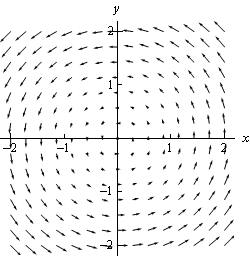
\includegraphics[width=8cm]{images/vec_field2.png}
\end{figure}
\end{proof}

\begin{defn}{Gradient vector}{}
Given a function $f(x,y,z)$, the gradient vector is defined by
\begin{equation}
\nabla f = \left\langle {{f_x},{f_y},{f_z}} \right\rangle
\end{equation}
This is a vector field and is often called a gradient vector field.
\end{defn}

\subsection{Types of line integrals}

\subsection{Fundamental Theorem for Line Integrals}
\begin{thrm}{Fundamental Theorem of Line Integrals}{}
Suppose that $C$ is a smooth curve from points $A$ to $B$ parameterised by $\vb{r}(t)$ for $t\in[a,b]$. Let $f$ be a differentiable function whose domain includes $C$ and whose gradient vector $\nabla f$ is continuous on $C$. Then
\begin{equation}
\int_C \nabla f \dd{\vb{r}} = f(\vb{r}(b)) - f(\vb{r}(a)) = f(B) - f(A)
\end{equation}
\end{thrm}
\begin{remark}
Similar to the fundamental theorem of calculus, the primary change is that gradient $\nabla f$ takes the place of the derivative $f^\prime$.
\end{remark}
% https://www.math.uci.edu/~ndonalds/math2e/16-3fundthm.pdf
% https://www.youtube.com/watch?v=_60sKaoRmhU

\subsection{Conservative Vector Fields}

\subsection{Green's Theorem}


to compute arc lengths, areas of curves 

applications of integrals to find area and volume

\chapter{Fourier Analysis}

\textbf{What is fourier analysis?}

Fourier analysis is the study of how general functions can be decomposed into trigonometric or exponential functions with definite frequencies. There are two types of Fourier expansions:

\begin{itemize}
\item Fourier series: If a (reasonably well-behaved) function is periodic, then it can be written as a discrete sum of trigonometric or exponential functions with specific frequencies.
\item Fourier transform: A general function that is not necessarily periodic (but that is still reasonably well-behaved) can be written as a continuous integral of trigonometric or exponential functions with a continuum of possible frequencies.
\end{itemize}

% https://scholar.harvard.edu/files/david-morin/files/waves_fourier.pdf
% https://math.mit.edu/~gs/cse/websections/cse41.pdf

\section{Fourier Trigonometric Series}
\textbf{Fourier's theorem} states that any (reasonably well-behaved) function can be written in terms of trigonometric or exponential functions, which we will eventually prove this theorem later. What we will do is derive what the coefficients of the sinusoidal functions must be, under the assumption that any function can in fact be written in terms of them.

Consider a function $f(x)$ that is periodic on the interval $0 \le x \le L$. Fourier's theorem works even if $f(x)$ is not continuous, although an interesting thing happens at the discontinuities, which we will talk about later. Other conventions for the interval are $-L \le x \le L$, or $0 \le x \le 1$, or $-\pi \le x \le \pi$, etc. There are many different conventions, but they all lead to the same general result in the end. If we assume $0 \le x \le L$ periodicity, then Fourier's theorem states that $f(x)$ can be written as

\begin{equation}\label{fourier_trigo}
f(x) = a_0 + \sum_{n=1}^\infty \sqbrac{a_n\cos\brac{\frac{2\pi nx}{L}+b_n\sin\brac{\frac{2\pi nx}{L}}}}
\end{equation}

where coefficients $a_i$ and $b_i$ take on certain values that we will calculate below. This expression is the \vocab{Fourier trigonometric series} for the function $f(x)$. We could alternatively not separate out the $a_0$ term, and instead let the sum run from $n=0$ to $\infty$, because $cos(0) = 1$ and $sin(0) = 0$. But the normal convention is to isolate the $a_0$ term.

With the $2\pi$ included in the arguments of the trig functions, the $n=1$ terms have period $L$, the $n=2$ terms have period $\frac{L}{2}$, and so on. So for any integer $n$, an integral number of oscillations fit into the period $L$. The expression in \cref{fourier_trigo} therefore has a period of (at most) $L$, which is a necessary requirement, of course, for it to equal the original periodic function $f(x)$. The period can be shorter than $L$ if, say, only the even n's have non-zero coefficients (in which case the period is L/2). But it can't be longer than L; the function repeats at least as often as with period L.

We're actually making two statements in \cref{fourier_trigo}. The first statement is that any periodic function can be written this way. This is by no means obvious, and it is the part of the theorem that we're accepting here. The second statement is that coefficients $a_i$ and $b_i$ take on particular values, assuming that the function f(x) can be written this way. It's reasonably straightforward to determine what these values are, in terms of f(x), and we'll do this below. But we'll first need to discuss the concept of orthogonal functions.

\section{Fourier Exponential Series}

\section{Fourier Transform}

\section{Special functions}
\subsection{Gaussian}
\subsection{Exponential, Lorentzian}
\subsection{Square wave, sinc}

\section{The delta function}

\section{Gibbs phenomenon}

\section{Convergence}

\section{Relation between transforms and series}

\part{Differential Geometry}
\textbf{Readings:}
\begin{itemize}
\item \href{https://aetemad.iut.ac.ir/sites/aetemad.iut.ac.ir/files/files_course/william_m._boothby_an_introduction_to_differentibookfi.org_.pdf}{Introduction to Differentiable Manifolds and Riemannian Geometry}
\item \href{http://www2.ing.unipi.it/griff/files/dC.pdf}{Differential Geometry of Curves and Surfaces}
\end{itemize}